%!TEX root=masterproef.tex
\subsection{Attesteren van software}
\label{subsection:attestation}

Het voorbeeld uit sectie \ref{section:node-capture} toonde al aan dat zelfs het
vluchtige geheugen van een knoop niet veilig is. Als een aanvaller in staat is
om ongemerkt de programma-code van een knoop te bekomen, alsook alle gegevens
die alleen tijdens uitvoering in het geheugen, dan kan deze aanvaller deze code
aanpassen zodat de werking ogenschijnlijk ongewijzigd is, maar dat hij toch
controle heeft over de werking en zo het hele netwerk kan be\"invloeden.

Een zeer logische onderzoeksvraag dient zich al snel aan: ``\emph{Is het
mogelijk om wijzigingen aan het programma van een knoop in het netwerk vast te
stellen?}''. Deze vraag wordt onderzocht binnen het domein van software
attestatie.

\cite{castelluccia2009difficulty} geeft enerzijds een goed overzicht van de
concepten evenals de mogelijkheden, maar vooral de moeilijkheden en beperkingen
van software attestatie.

\subsubsection*{Werking}

Alle bestaande vormen van software attestatie maken gebruik van een protocol
gebaseerd op het challenge response principe. Als men de integriteit van een
knoop wil vast stellen, zal men aan deze knoop een verzoek sturen om een unieke
samenvatting te maken van zijn inhoud door middel van een cryptografische
hashfunctie, een \emph{checksum}.

De vaststeller beschikt zelf over een versie van de inhoud van de knoop en kan
dezelfde unieke samenvatting berekenen. Door in het initi\"ele verzoek een
\'e\'enmalig te gebruiken code mee te geven, een zgn. \emph{nonce}, en deze
deel te laten uitmaken van de inhoud, kunnen verschillende verzoeken telkens
met een ander, unieke samenvatting beantwoord worden en wordt kan deze
samenvatting niet op voorhand gekend en berekend worden. Figuur
\ref{fig:attestation-process} geeft een overzicht van de werking van software
attestatie en illustreert hoe een wijziging door een aanvaller zich propageert.

\begin{figure}
  \centering
  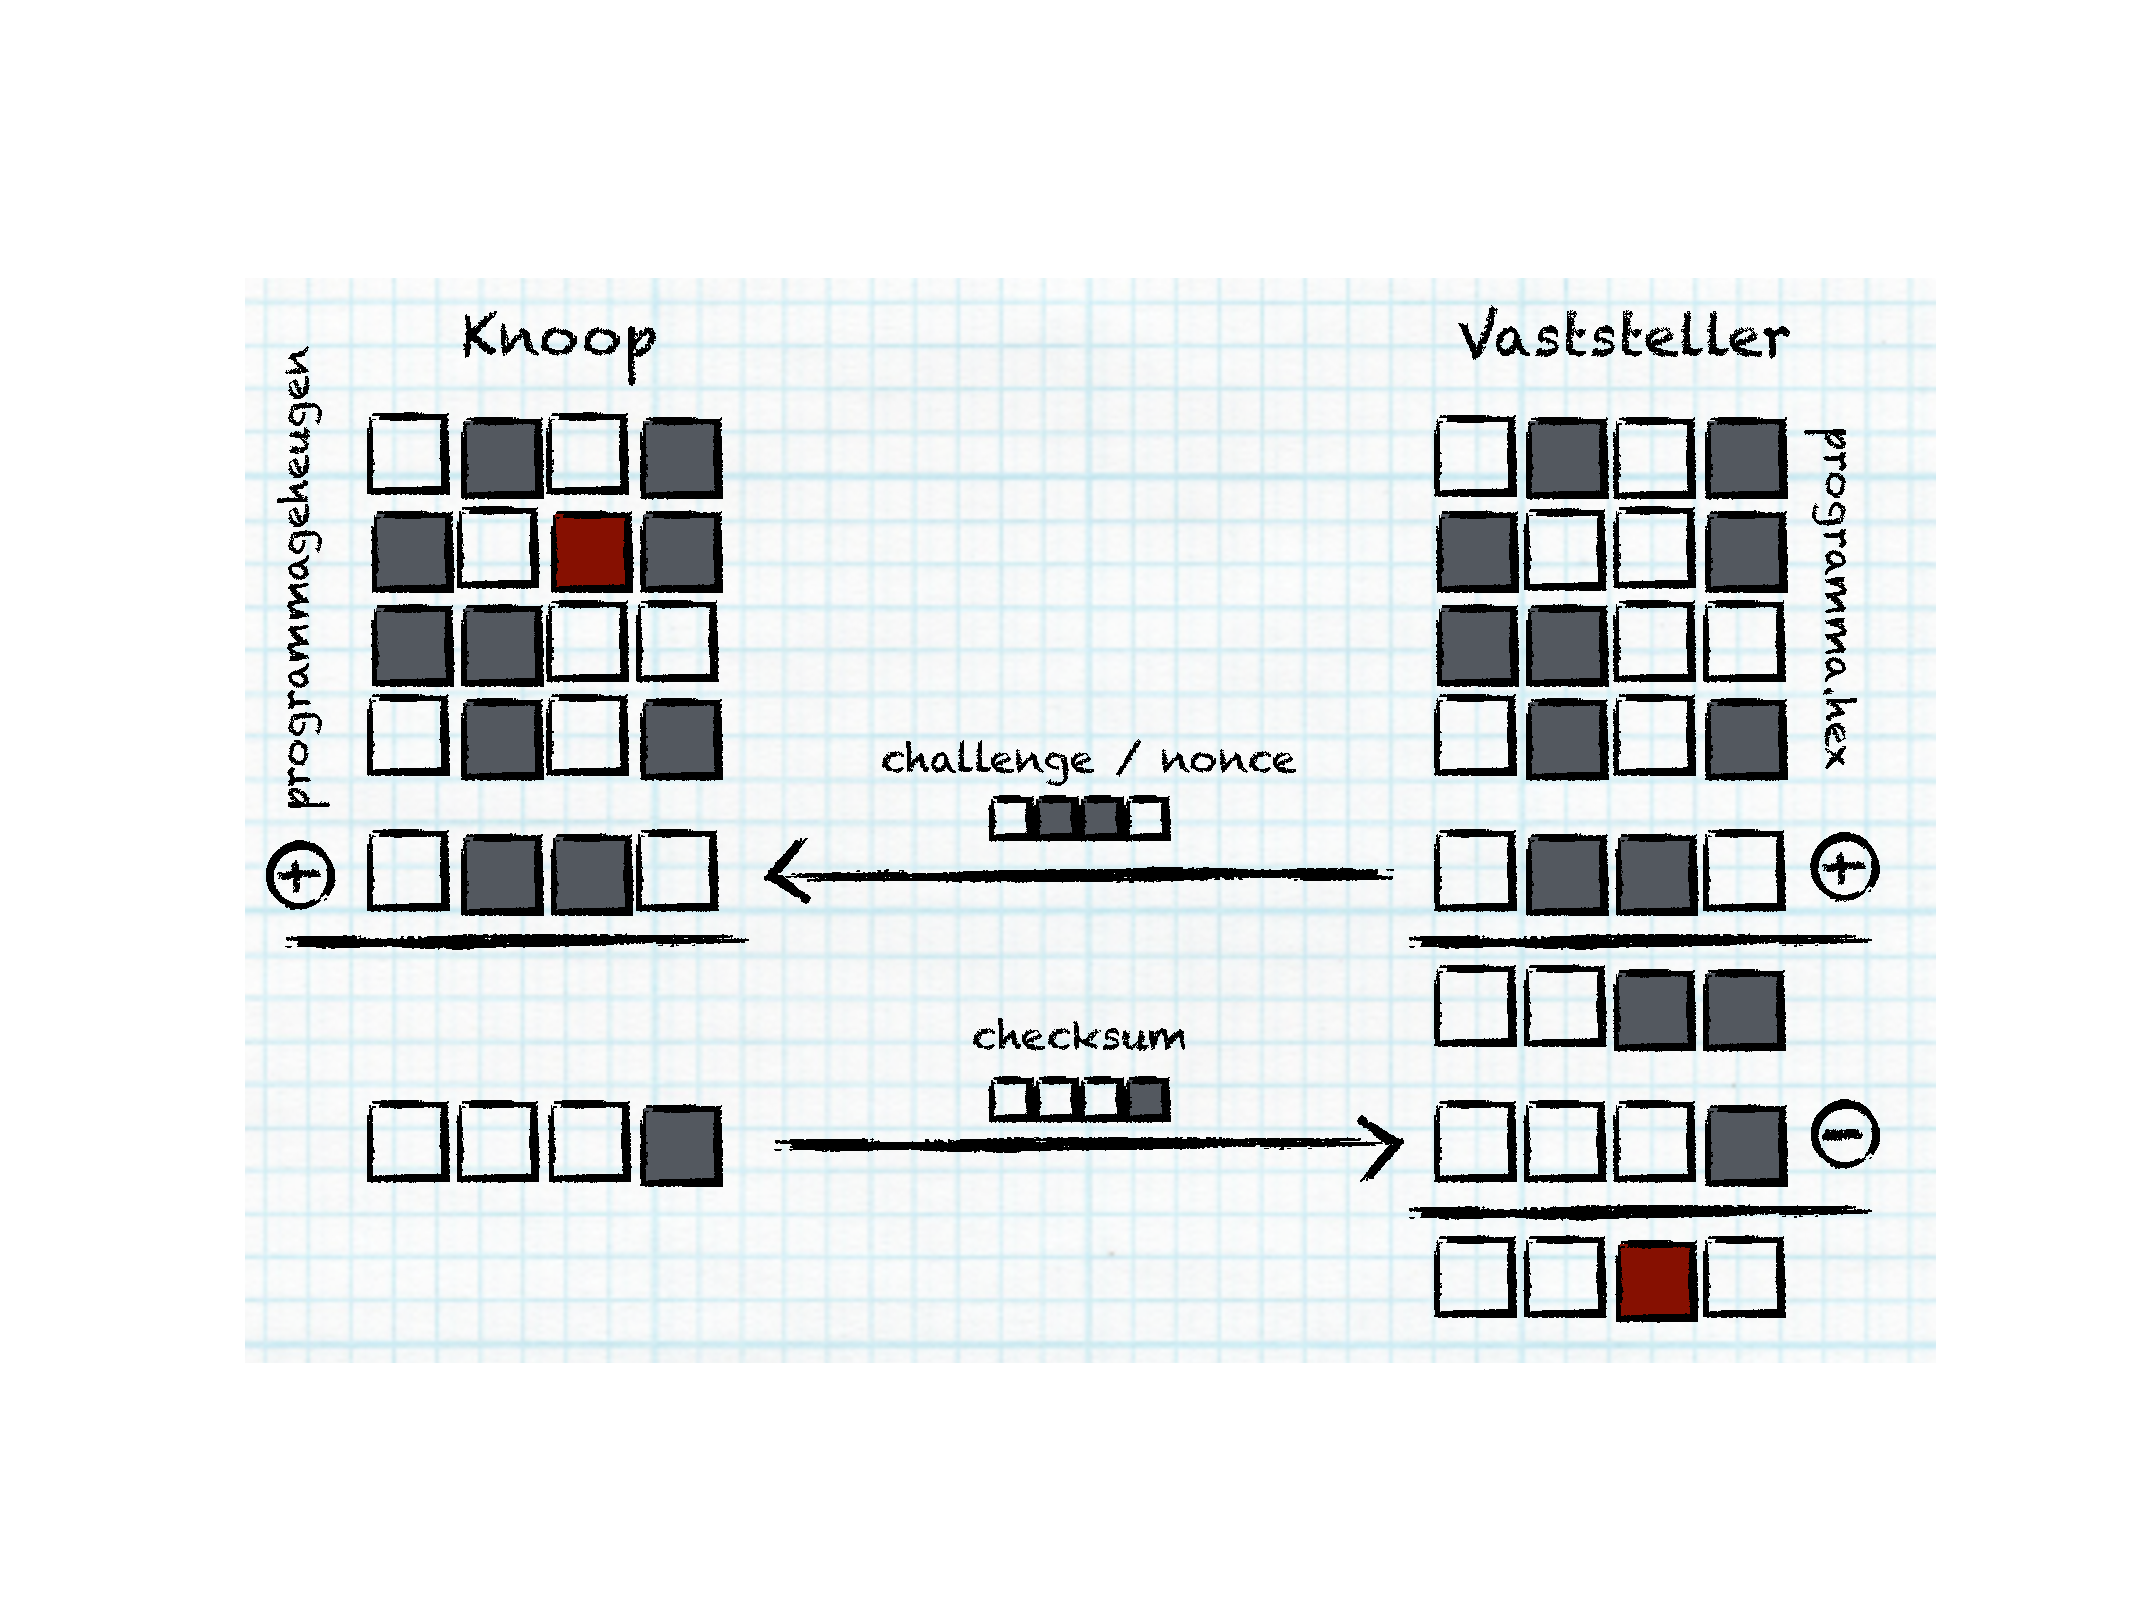
\includegraphics[width=0.9\linewidth]{resources/attestation-process.pdf}
  \caption{De werking van software attestatie: een aanvaller heeft een
  wijziging kunnen aanbrengen in de programma code op een knoop. Deze wijziging
  propageert zich in de \emph{checksum} en wordt door de vaststeller opgemerkt.}
  \label{fig:attestation-process}
\end{figure}

De inhoud waarvan een samenvatting gemaakt wordt is typisch de programma code
die op de knoop ge\"installeerd werd. Indien een aanvaller deze code kon
wijzigen, zou de samenvatting niet langer overeenkomen met die opgesteld door
de vaststeller en kan deze laatste besluiten om deze gewijzigde code niet te
vertrouwen en de knoop uit te sluiten.

\subsubsection*{Aanvalsmogelijkheden}

Ondanks de mogelijkheden zijn er spijtig genoeg verschillende manieren om deze
vorm van integriteit-controle te omzeilen.

De eenvoudigste manier om de attestatie code te omzeilen bestaat er in om de
opgevraagde geheugenadressen te controleren en indien ze verwijzen naar
plaatsen waar zich niet-originele code bevindt, deze te herschrijven naar
adressen waar de originele code zich bevindt.

Aangezien het merendeel van het programma geheugen op een knoop typisch leeg
is, kan de aanvaller zijn benodigde code verbergen in zo'n stuk leeg geheugen.
Mits zorgvuldige keuze van deze locatie, kan het controleren van en verwijzen
naar een andere locatie zich beperken tot de manipulatie van \'e\'en enkele bit
in het adres. Deze techniek wordt ook wel een geheugen schaduwende aanval
genoemd.

Om het probleem van leeg programma geheugen en de bijhorende uitnodiging aan
het adres van de aanvaller om zich eenvoudig te kunnen verschuilen, aan te
pakken, stelt o.a. \cite{yang2007distributed} voor om dit geheugen voor dat het
op een knoop wordt geplaatst, op te vullen met willekeurige waarden. Op deze
manier heeft de aanvaller geen vrije ruimte om zijn code in te plaatsen.

Ofschoon deze willekeurige data inderdaad zo kan opgesteld worden dat ze niet
kan verkleind worden, kan dit niet gegarandeerd worden van de eigenlijke
programma code. Deze kan typisch wel nog verkleind worden en in die vorm
opgeslagen worden, waardoor er ruimte vrijkomt voor de code van de aanvaller.
Op het ogenblik van attestatie kan deze oorspronkelijke code dan, indien nodig
terug hersteld worden.

Indien deze eenvoudige technieken toch niet voldoende ruimte zouden bieden, kan
er nog altijd gekeken worden naar het data geheugen. We merken immers op dat
nagenoeg alle vormen van attestatie alleen toegepast worden op het programma
geheugen. Het data geheugen is immers te veranderlijk en kan niet volledig
gekend zijn door de vaststeller.

Hierdoor wordt dit data geheugen natuurlijk het volgende aandachtspunt voor de
aanvaller. Ondanks het feit dat ook op een \mcu het data geheugen veelal niet
kan uitgevoerd worden, blijft het mogelijk om programma code in het data
geheugen op te slagen en te kopi\"eren naar het programma geheugen.

De \emph{rootkit} voorgesteld in \cite{castelluccia2009difficulty} hanteert dit
principe. Door middel van de \emph{Return Operation Programming} (ROP)
techniek, o.a. beschreven in \cite{prandini2012return}, kan een aanvaller met
eerste haak bij aanvang van de attestatie code in het programma geheugen, zijn
eigen rootkit uit het programma geheugen laten verwijderen. Na deze operatie is
het programma geheugen opnieuw intact en zal de originele attestatie routine
een positief resultaat opleveren. Maar de eerste haak heeft er ook voor gezorgd
dat de bij terugkeer uit de attestatie routine een tweede haak geplaatst is die
op zijn beurt de rootkit en de initi\"ele haak opnieuw door middel van ROP
instructies installeert. Figuur \ref{fig:attestation-rootkit} toont deze
werking.

\begin{figure}
  \centering
  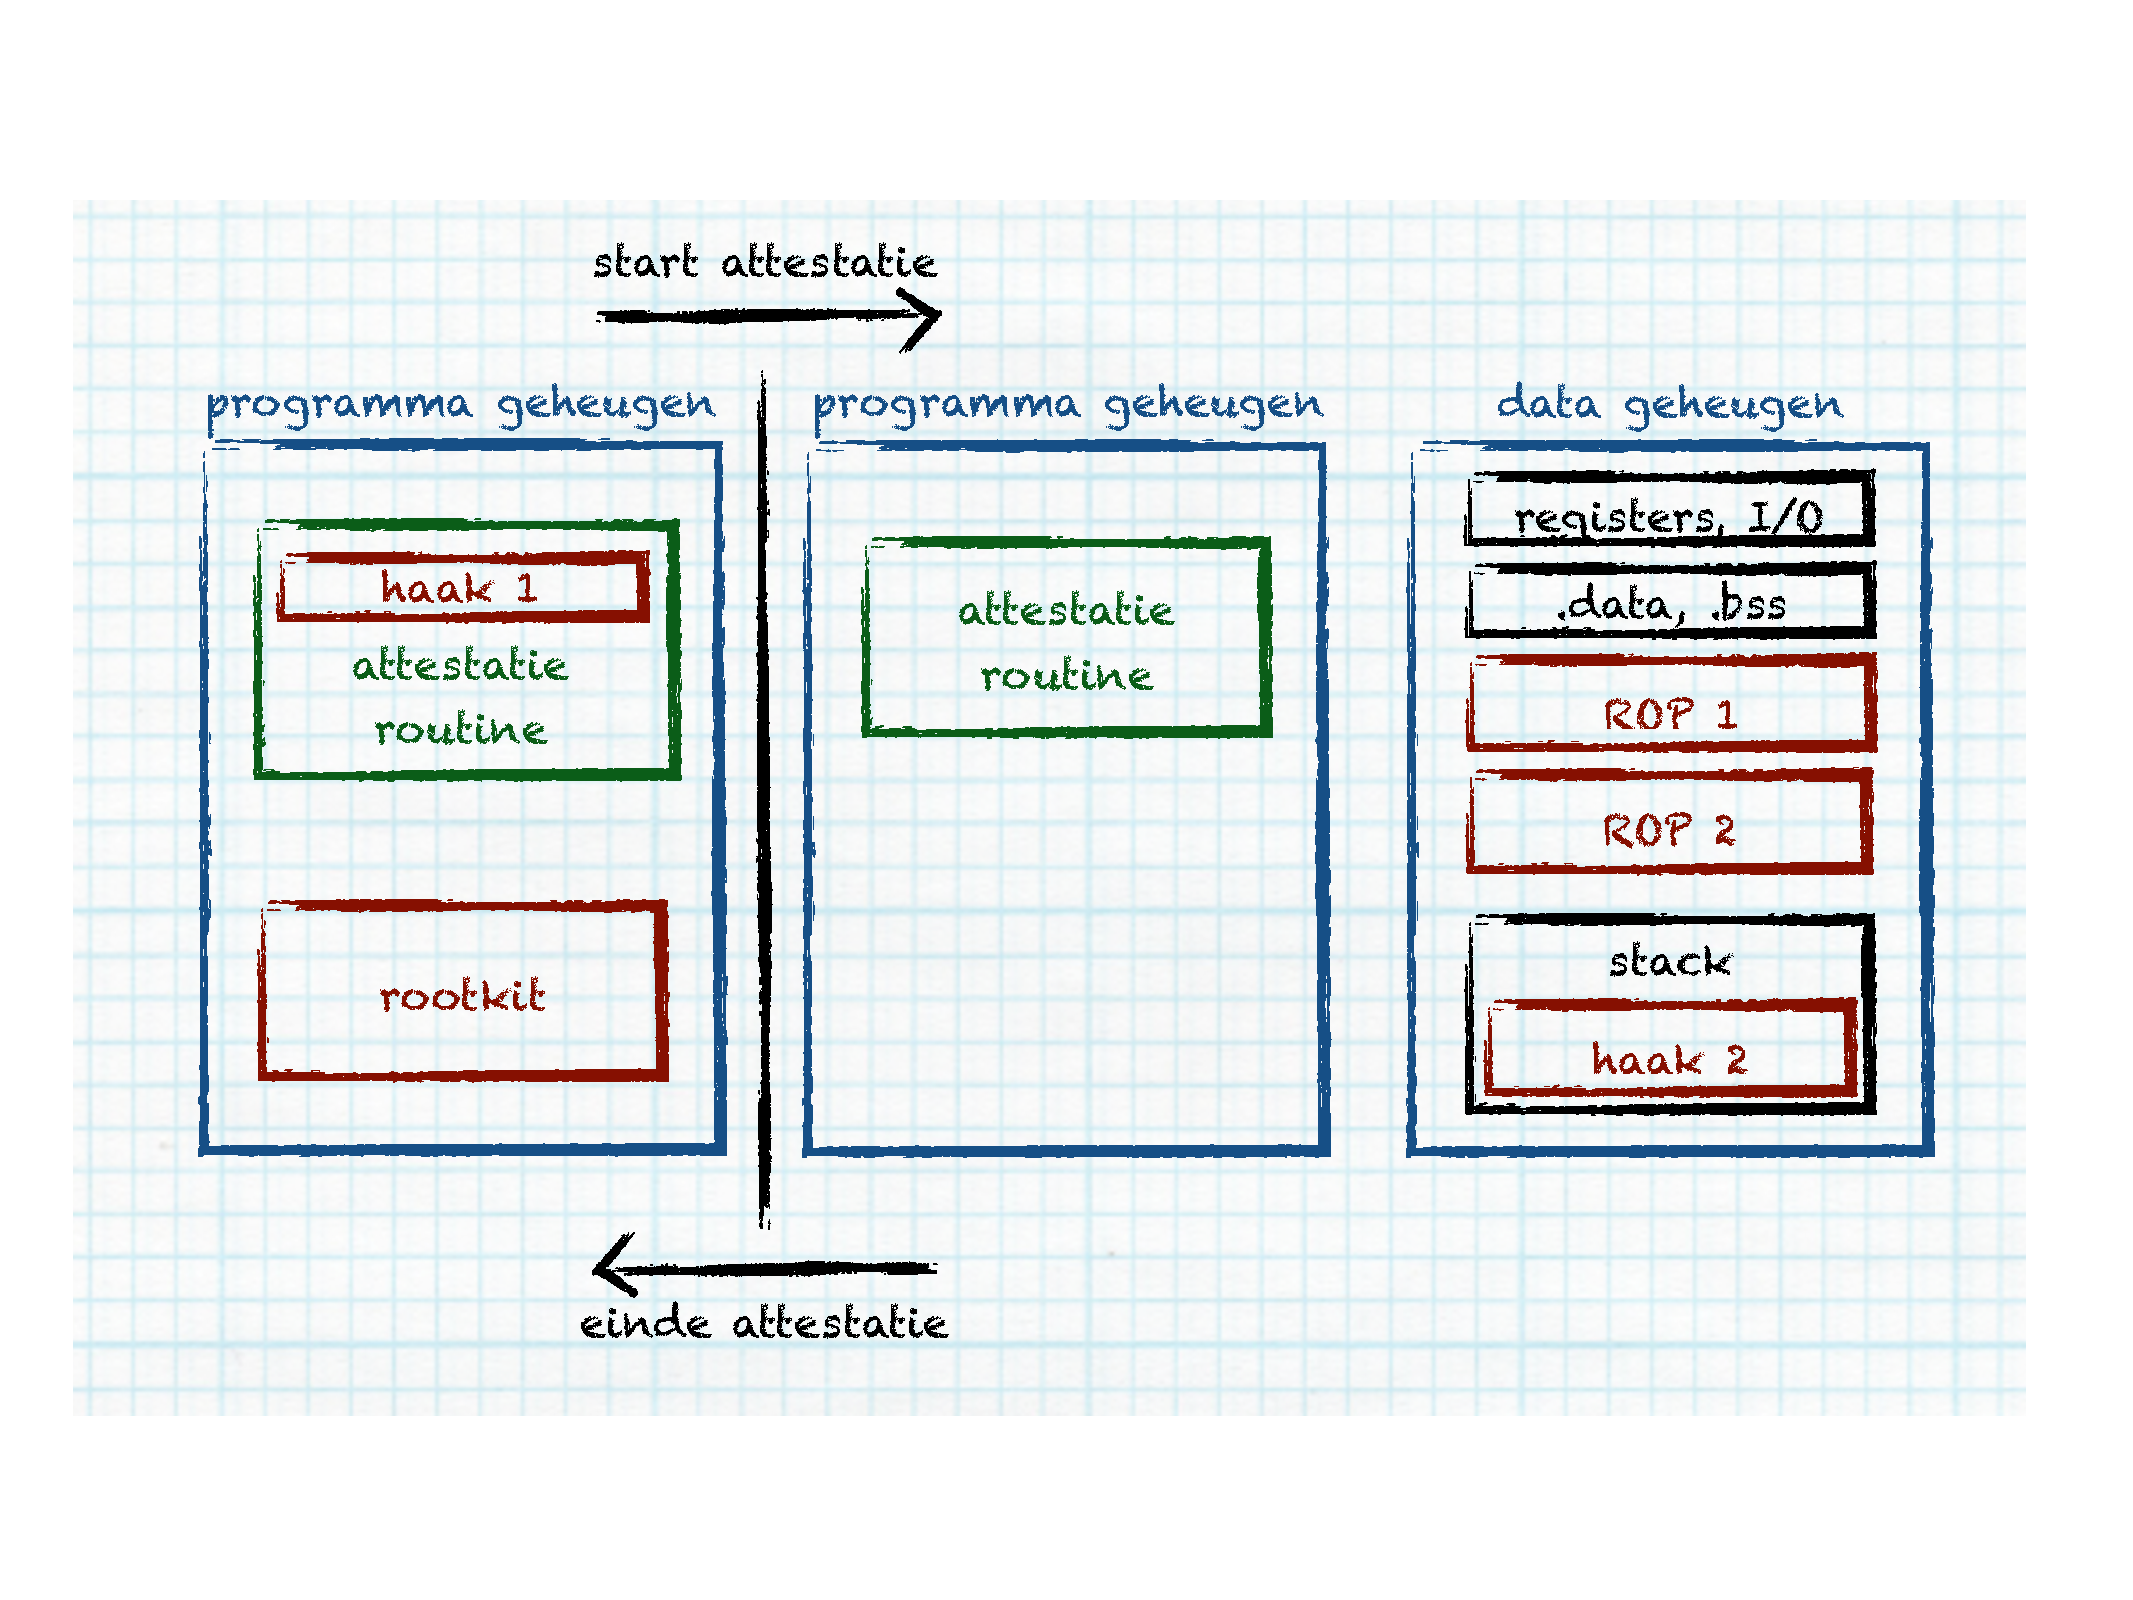
\includegraphics[width=0.9\linewidth]{resources/attestation-rootkit.pdf}
  \caption{De werking van een attestatie ontwijkende rootkit.}
  \label{fig:attestation-rootkit}
\end{figure}

Het verbergen van de rootkit en het herstellen van het programma geheugen in
zijn oorspronkelijke staat blijkt slechts een overhead van ongeveer 0.3\% op te
leveren t.o.v. bv. de SWATT attestatie techniek voorgesteld in
\cite{seshadri2004swatt}. Deze techniek controleert tevens de tijd dat de
attestatie routine nodig had om de checksum te berekenen. Indien deze te lang
duurt dan schrijft SWATT dit toe aan de overhead ge\"introduceerd door
mogelijke kwaadaardige code. Een verhoging met 0.3\% is te weinig om tot deze
conclusie te komen.

Een attestatie routine zou zichzelf kunnen beschermen tegen een dergelijke
rootkit door op het einde van zijn implementatie het data geheugen volledig
leeg te maken en vervolgens, zonder een terugkeer operatie uit te voeren
waardoor de tweede haak vermeden wordt, de knoop te herstarten. Het verwijderen
van alle gegevens en het herstarten van een knoop bij elk attestatie verzoek,
kan afhankelijk van de functionaliteit die de knoop aanbiedt, in de meeste
gevallen niet wenselijk zijn. Dit euvel kan eventueel wel ondervangen worden
door het wegschrijven van deze gegevens naar een EEPROM.

Een andere oplossingsstrategie zou kunnen liggen in het attesteren van het data
geheugen. Dit moet dan wel op op het zelfde ogenblik gebeuren als de attestatie
van het programma geheugen, zodat de rootkit niet in staat is om zichzelf heen
en weer te kopi\"eren tussen de twee afzonderlijke attestaties. Zelfs al wordt
er willekeurig telkens uit het ene of het andere geheugen gelezen, dan nog kan
de rootkit zich nog steeds verplaatsen tussen de twee geheugens en moet deze
dat dan zelfs maar gemiddeld om de twee lees operaties doen. Hierdoor zal de
overhead zelfs gedeeld door twee worden, waardoor de impact ervan nog
moeilijker te detecteren wordt.

Tot slot is, zoals eerder reeds vermeld, het attesteren van het werkgeheugen op
zich reeds een zeer moeilijk gegeven, door de onvoorspelbare inhoud ervan.
Idealiter zou de vaststeller ook de inhoud van het volledige data geheugen
moeten kennen. Enerzijds bevat dit geheugen registers enz., welke volledig
onvoorspelbaar zijn en dus uitgesloten zouden moeten worden. Anderzijds bevat
het geheugen gegevens van de actieve processen. Deze zijn typisch afhankelijk
van opgemeten waarden en/of communicatie met andere knopen en dus per definitie
onvoorspelbaar voor de vaststeller.

Opnieuw zou het leegmaken van het data geheugen een voorspelbaar resultaat
opleveren voor de vaststeller, maar dit is dan evengoed een voorspelbaar
resultaat voor de aanvaller en kunnen opnieuw geheugen schaduwende technieken
gebruikt worden.

\subsubsection*{Conclusies en gevolgen}

Uit voorgaande paragrafen kunnen we vaststellen dat het op een eenvoudige \mcu
nagenoeg onmogelijk is om een sluitende oplossing voor software attestatie uit
te realiseren omdat de code van een aanvaller zich steeds tussen de
verschillende stappen in de attestatie procedure kan wringen. Zelfs indien de
vaststeller rekening houdt met de tijd die de knoop nodig heeft om de
attestatie te voltooien, zijn er technieken die snel genoeg zijn om ook hier
binnen de aannemelijke grenzen te vallen.



\subsubsection*{Potentieel}

-> AMI situatie \cite{lemay2012cumulative}

\TODO
